\chapter{Stato dell'arte}
Data la rapida evoluzione nel campo della visione artificiale, l'analisi dello
stato dell'arte risulta fondamentale per identificare le metodologie più
promettenti volte a coniugare elevate prestazioni e sostenibilità
computazionale. In questo capitolo verrà esaminato il panorama delle soluzioni
atte a rendere i \textbf{Vision Transformer} (ViT) applicabili in scenari
reali, caratterizzati da vincoli di latenza, memoria e consumo energetico.
Notare che nessuna soluzione esclude automaticamente le altre, spesso molti di
questi approcci vengono integrati e combinati per ottenere risultati migliori.
\begin{figure}[H]
    \centering
    \includegraphics[width=0.75\textwidth]{images/SOTA/tassonomia.pdf}
    \caption{Tassonomia delle principali metodologie per l'efficientamento dei modelli di visione artificiale.}
\end{figure}
La trattazione si articolerà su due fronti principali:
\begin{itemize}
    \item \textbf{Ottimizzazione Architetturale:} l'analisi di modelli e architetture appositamente progettate per ridurre la complessità computazionale, i costi di memoria o anche i consumi energetici dell'inferenza.
          \begin{itemize}
              \item \textbf{Architetture Ibride:} si tratta di architetture che integrano elementi tipici dei modelli \textit{Transformer} con elementi tipici delle reti convoluzionali, al fine di sfruttare i punti di forza di entrambe le tipologie di modelli e ottenere un buon compromesso tra prestazioni e efficienza;
              \item \textbf{Architetture Edge-Optimized}: modelli progettati specificamente per essere eseguiti su dispositivi con risorse limitate, come smartphone o dispositivi IoT, con l'obiettivo di massimizzare le prestazioni mantenendo un basso consumo energetico e ridotti requisiti computazionali.
              \item \textbf{Neural Architecture Search (NAS):} ovvero l'automazione del processo di design di architetture ottimali in termini di costi e prestazioni.
          \end{itemize}
    \item \textbf{Tecniche di Compressione dei modelli:} lo studio di metodologie applicabili a reti pre-esistenti al fine di ridurne la dimensione e migliorarne l'efficienza, tra cui:
          \begin{itemize}
              \item \textbf{Pruning:} ovvero la rimozione di pesi, teste di attenzione o interi blocchi ridondanti dall'architettura per snellire il modello senza compromettere significativamente le prestazioni;
              \item \textbf{Quantizzazione:} cioé la riduzione della precisione numerica della rappresentazione dei parametri, ottenendo modelli molto più compatti in termini di memoria e veloci da eseguire su hardware specializzato;
              \item \textbf{Knowledge Distillation:} il trasferimento di conoscenza da modelli \textit{teacher} grandi e complessi a modelli \textit{student} più piccoli e leggeri, aumentando in modo importante le prestazioni ottenibili da questi ultimi;

          \end{itemize}
\end{itemize}
\section{Architetture efficienti di ViT}
\subsection{Architetture Ibride}
A partire dall'introduzione dei \textit{Vision Transformer} (ViT) da parte di
Dosovitskiy et al.\cite{dosovitskiy2021imageworth16x16words}, numerosi sforzi
sono stati fatti per sviluppare architetture che potessero mantenere le
prestazioni elevate dei ViT, ma con una complessità computazionale ridotta. Tra
queste, le architetture ibride rappresentano una delle direzioni più
promettenti ed esplorate.
\subsubsection{BoTNet}
Uno dei primi approcci è stato quello presentato da Srinivas et
al.\cite{srinivas2021bottlenecktransformersvisualrecognition}, nel quale è
stata modificata una architettura ResNet \cite{he2015deepresiduallearningimage}
sostituendo le convoluzioni spaziali $(3x3)$ negli ultimi 3 blocchi (definiti
\textit{bottleneck}) con delle Multi-Head Self-Attention.
\begin{figure}[H]
    \centering
    \includegraphics[width=0.6\textwidth]{images/SOTA/BoTNet.pdf}
    \caption{Confronto tra il blocco ResNet e il blocco BoTNet. Fonte: \cite{srinivas2021bottlenecktransformersvisualrecognition}.}
\end{figure}
In particolare questa architettura ha dimostrato delle performance migliori rispetto alla ResNet-50, con un numero di parametri simile, ma con una complessità computazionale più elevata, data dall'introduzione dell'attenzione. Questo lavoro ha dimostrato che l'integrazione delle due architetture è una direzione di ricerca promettente, ma è necessario trovare un compromesso tra prestazioni e complessità computazionale.
\subsubsection{CvT}
I pionieri dell'applicazione delle convoluzioni ad un ViT sono stati Wu et.
al\cite{wu2021cvtintroducingconvolutionsvision}, con il loro
\textbf{Convolutional Vision Transformer}, che ha introdotto delle convoluzioni
per produrre le query, key e value all'interno di nuovi \textit{Convolutional
    Transformer Block}, integrando profondamente le due architetture. Questo tipo
di approccio ha eliminato la necessità del \textit{Positional Encoding} tramite
le proprietà delle convoluzioni.
\begin{figure}[H]
    \centering
    \includegraphics[width=0.8\textwidth]{images/SOTA/cvt.pdf}
    \caption{A sinistra l'architettura CvT, a destra la struttura del blocco \textit{Convolutional Transformer}. Fonte: \cite{wu2021cvtintroducingconvolutionsvision}.}
\end{figure}
Questo tipo di soluzione ha permesso di raggiungere ottime performance su vari task, mantenendo contenuto il numero di parametri.
\subsubsection{CoAtNet}
Un ulteriore pilastro di questo approccio ibrido è quello di Dai et
al.\cite{dai2021coatnetmarryingconvolutionattention}, i quali hanno proposto
un'architettura CNN-\textit{Transformer} definita \textbf{Co-AtNet}, con
l'obiettivo di sfruttare i punti di forza delle due architetture. In
particolare, gli autori hanno combinato blocchi convoluzionali
\textit{Depthwise} e moduli di \textit{Self-Attention} organizzandoli in stadi
successivi, con l'obiettivo di ridurre la complessità computazionale mantenendo
elevate prestazioni.
\begin{figure}[H]
    \centering
    \includegraphics[width=0.85\textwidth]{images/SOTA/coatnet_arch.pdf}
    \caption{L'architettura di CoAtNet.Fonte: \cite{dai2021coatnetmarryingconvolutionattention}.}
\end{figure}
Gli autori hanno dimostrato che questo approccio permette di raggiungere prestazioni superiori rispetto a molte architetture CNN e ViT, con un numero di parametri e un numero di operazioni in virgola mobile inferiori.
\subsubsection{FastViT}
Di recente, ulteriori sviluppi sono stati presentati da Vasu et al.
\cite{vasu2023fastvitfasthybridvision} con l'architettura \textbf{FastViT},
nella quale si affronta il problema della latenza causata dai frequenti accessi
in memoria necessari durante l'inferenza. In particolare, le connessioni
residuali, seppur fondamentali per evitare la scomparsa del gradiente,
contribuiscono pesantemente a questo problema, richiedendo di recuperare
continuamente dalla memoria i valori sui quali eseguire la somma.
\begin{figure}[H]
    \centering
    \includegraphics[width=0.9\textwidth]{images/SOTA/fastvit_arch.pdf}
    \caption{L'architettura del modello FastViT. Fonte: \cite{vasu2023fastvitfasthybridvision}.}
\end{figure}
Gli autori risolvono questo problema applicando una \textbf{riparametrizzazione strutturale post-addestramento} all'interno di un modulo proprietario denominato \textbf{RepMixer}. Durante il \textit{training}, la rete sfrutta connessioni residuali e convoluzioni su rami paralleli per massimizzare la capacità di apprendimento; in fase di inferenza, queste strutture parallele vengono fuse matematicamente in un'unica convoluzione di tipo \textit{depthwise}. Questo approccio permette di eliminare del tutto le operazioni di somma e i relativi accessi in memoria, mantenendo inalterate le elevate prestazioni predittive.
Infine, sebbene l'architettura di \textit{FastViT} affidi i primi tre stadi interamente a operazioni convoluzionali per abbattere rapidamente la risoluzione, nell'ultimo stadio viene introdotta la \textit{Self-Attention}. Questa scelta strategica permette di ampliare il \textit{receptive-field} e catturare le dipendenze globali solo quando la mappa delle \textit{feature} è sufficientemente ridotta, evitando un aumento eccessivo della complessità computazionale. Grazie a queste soluzioni, il modello raggiunge prestazioni uguali o superiori alle architetture ibride di riferimento, ma con latenza e operazioni in virgola mobile (FLOPs) drasticamente inferiori.
\subsubsection{FasterViT}
Una ulteriore direzione di ricerca è quella di modificare il meccanismo di
attenzione, al fine di introdurlo in una architettura basata su CNN, per
limitare i costi introdotti. In questo senso Hatamizadeh et al.
\cite{hatamizadeh2024fastervitfastvisiontransformers} propongono l'architettura
\textbf{FasterViT}, nella quale viene introdotto un nuovo meccanismo di
attenzione, denominato \textbf{Hierarchical Attention}.
\begin{figure}[H]
    \centering
    \includegraphics[width=0.95\textwidth]{images/SOTA/fastervit_arch_horizontal.pdf}
    \caption{L'architettura del modello FasterViT. Fonte: \cite{hatamizadeh2024fastervitfastvisiontransformers}.}
\end{figure}
L'approccio proposto risulta particolarmente efficace nei casi in cui vengono elaborati input ad alta risoluzione, in queste situazioni il calcolo della \textit{Self-Attention} globale diventa rapidamente proibitivo a causa del suo costo computazionale quadratico. D'altra parte, limitare l'attenzione a finestre spaziali isolate (come avviene nello \textit{Swin Transformer}) comporta la perdita cruciale del contesto globale. Per superare questo ostacolo, gli autori propongono una macro-architettura ibrida strutturata in quattro stadi sequenziali. I primi due stadi operano esclusivamente tramite blocchi residui convoluzionali, i quali estraggono le \textit{feature} locali ed eseguono un sottocampionamento spaziale. Soltanto nel terzo e quarto stadio, dove la risoluzione delle \textit{feature map} risulta notevolmente ridotta, intervengono i moduli \textit{Transformer}.
\begin{figure}[H]
    \centering
    \includegraphics[width=0.2\textwidth]{images/SOTA/fastervit_HAT.pdf}
    \caption{Mappa di attenzione del meccanismo di \textit{Hierarchical Attention}. Fonte: \cite{hatamizadeh2024fastervitfastvisiontransformers}.}
\end{figure}
La vera innovazione di \textit{FasterViT} risiede nel nuovo meccanismo di \textbf{Hierarchical Attention (HAT)} utilizzato in questi ultimi stadi. Il modello introduce dei \textit{Carrier Tokens} (token portatori) che agiscono come ponte informativo: questi speciali \textit{token} riassumono prima le informazioni all'interno delle singole finestre locali, interagiscono poi tra di loro a livello globale scambiandosi il contesto generale dell'immagine e, infine, ritrasmettono l'informazione globale aggiornata ai \textit{token} delle rispettive finestre locali. Questo approccio si avvicina ad un concetto di un \textit{receptive-field} globale ma con una frazione del costo computazionale originale. Utilizzando queste novità \textit{FasterViT} riesce a stabilire nuovi standard di velocità ed efficienza, dimostrando che l'uso sinergico di convoluzioni iniziali e attenzione negli ultimi stadi è una strategia molto efficace per ottenere ottime prestazioni con costi computazionali contenuti.
\subsubsection{Vision Mamba}
Infine, negli ultimissimi anni, il concetto di ibridazione si è spinto oltre la
combinazione di CNN e \textit{Transformer} classici. Per far fronte alla
necessità di elaborare sequenze visive o immagini ad altissima risoluzione con
complessità strettamente lineare $\mathcal{O}(N)$, la ricerca più recente ha
iniziato a sostituire i moduli di attenzione globale con i Modelli a Spazio di
Stato (SSM), in particolare la loro declinazione denominata \textbf{Mamba}
\cite{gu2024mambalineartimesequencemodeling}.
\begin{figure}[H]
    \centering
    \includegraphics[width=0.9\textwidth]{images/SOTA/vision_mamba.pdf}
    \caption{Architettura di Vision Mamba. Fonte: \cite{zhu2024visionmambaefficientvisual}.}
\end{figure}
Architetture ibride emergenti, come le varianti convoluzionali di \textbf{Vision Mamba (Vim)} \cite{zhu2024visionmambaefficientvisual}, integrano l'estrazione di \textit{feature} locali tipica delle CNN con il ragionamento sequenziale bidirezionale degli SSM. Sebbene i ViT ibridi rimangano lo standard di fatto nell'industria odierna, questa nuova frontiera CNN-SSM rappresenta la naturale evoluzione per abbattere definitivamente il costo quadratico dell'attenzione.
\subsection{Architetture Edge-Optimized}
Uno dei principali ostacoli all'implementazione dei ViT in scenari reali è
rappresentato dalle grandi difficoltà nell'esecuzione su dispositivi con
risorse limitate, come smartphone o dispositivi IoT. Per affrontare questo
problema sono stati fatti dei grandi passi avanti sia in ambito hardware,
implementando acceleratori specializzati per l'esecuzione di modelli neurali
(NPU, \textit{Neural Processing Unit}), sia in ambito architetturale,
progettando modelli specificamente ottimizzati per i dispositivi \textit{edge}.
\subsubsection{MobileViT}
Uno dei primi lavori in questo senso è stato quello di Mehta et al.
\cite{mehta2022mobilevitlightweightgeneralpurposemobilefriendly}, con il famoso
\textbf{MobileViT} che utilizza un approccio ibrido per coniugare l'efficienza
computazionale delle CNN con la capacità di catturare dipendenze globali dei
ViT.
\begin{figure}[H]
    \centering
    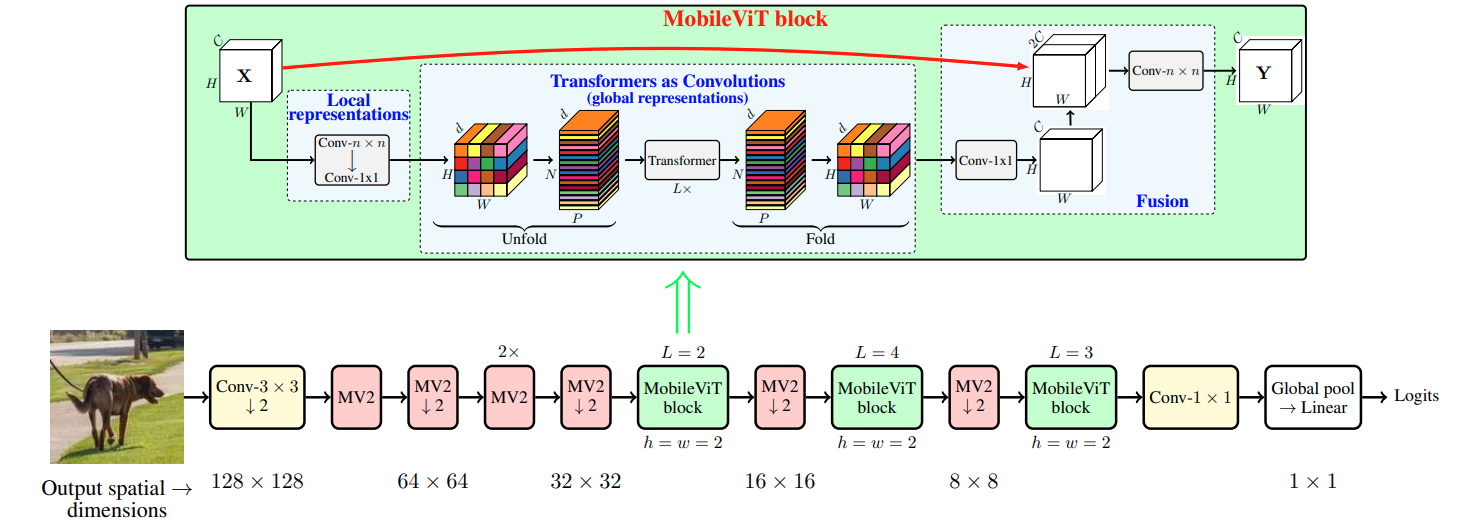
\includegraphics[width=0.95\textwidth]{images/SOTA/mobilevit_arch.png}
    \caption{Architettura di MobileViT. Fonte: \cite{mehta2022mobilevitlightweightgeneralpurposemobilefriendly}.}
\end{figure}
Scendendo in profondità, l'architettura di MobileViT è composta principalmente da blocchi MV2 (MobileNetV2 \cite{sandler2019mobilenetv2invertedresidualslinear}), che si occupano di eseguire il sottocampionamento e catturare le dipendenze locali, alternati da blocchi \textit{MobileViT}. Questi ultimi costituiscono il contributo più significativo di questo lavoro. A differenza dei classici \textit{Vision Transformer} che appiattiscono irrimediabilmente le singole \textit{patch} rovinando la topologia bidimensionale dell'immagine, i blocchi \textit{MobileViT} preservano la geometria spaziale elaborando le dipendenze globali in modo mirato.
\begin{figure}[H]
    \centering
    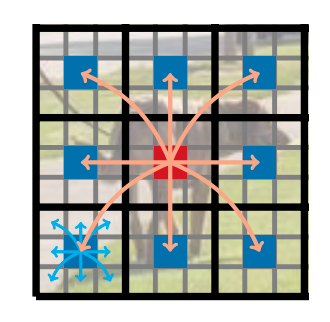
\includegraphics[width=0.3\textwidth]{images/SOTA/mobilevit_attn.png}
    \caption{Meccanismo di attenzione di MobileViT. Fonte: \cite{mehta2022mobilevitlightweightgeneralpurposemobilefriendly}.}
\end{figure}
Per ottenere questo risultato, il blocco esegue un'operazione matematica che
gli autori definiscono \textit{unfolding} (srotolamento). La mappa delle
\textit{feature} viene idealmente divisa in piccole finestre, o \textit{patch}.
Per costruire le sequenze monodimensionali rigorosamente richieste dal
\textit{Transformer}, il modello non fonde i pixel della singola
\textit{patch}, ma estrae esclusivamente i pixel che occupano la stessa posizione spaziale all'interno di tutte le \textit{patch}
dell'immagine (ad esempio, raggruppando tutti i pixel in alto a sinistra di
ogni finestra). Ognuno di questi pixel estratti rappresenta un singolo
\textit{token}. L'insieme di questi pixel omologhi forma la sequenza su cui viene calcolata la
\textit{Self-Attention}. Questo approccio si rivela vincente perché permette di
ottenere un campo recettivo globale a livello di singolo pixel senza pagarne il
reale prezzo computazionale. Infatti, calcolare un'attenzione globale su tutti
i pixel dell'immagine contemporaneamente comporterebbe un costo elevatissimo, insostenibile per un dispositivo mobile; calcolandola invece in parallelo su
queste specifiche sotto-sequenze posizionali, il costo totale viene abbattuto
drasticamente. Terminato il calcolo dell'attenzione, entra in gioco
l'operazione inversa, definita \textit{folding} (ripiegamento). I pixel appena
aggiornati dal \textit{Transformer} vengono ricollocati nelle
loro coordinate 2D di origine, restituendo in uscita una mappa spaziale intatta
e pronta per le elaborazioni successive.
Tramite questo approccio, MobileViT raggiunge e supera le prestazioni sia delle CNN, che dei ViT tradizionali, risultando più efficiente di questi ultimi ma non delle prime.
\subsubsection{Mobile-Former}
In \cite{chen2022mobileformerbridgingmobilenettransformer}, Chen et al. propongono un'architettura innovativa che integra le due architetture \textit{MobileNet} e \textit{Transformer} in modo più profondo rispetto a MobileViT. In particolare, introducono un nuovo modulo, denominato \textbf{Mobile-Former Block}, che prevede due rami paralleli, uno convoluzionale (ispirato alla \textit{MobileNet}) e uno basato su attenzione, con connessioni bidirezionali che permettono uno scambio continuo di informazioni tra i due rami.
\begin{figure}[H]
    \centering
    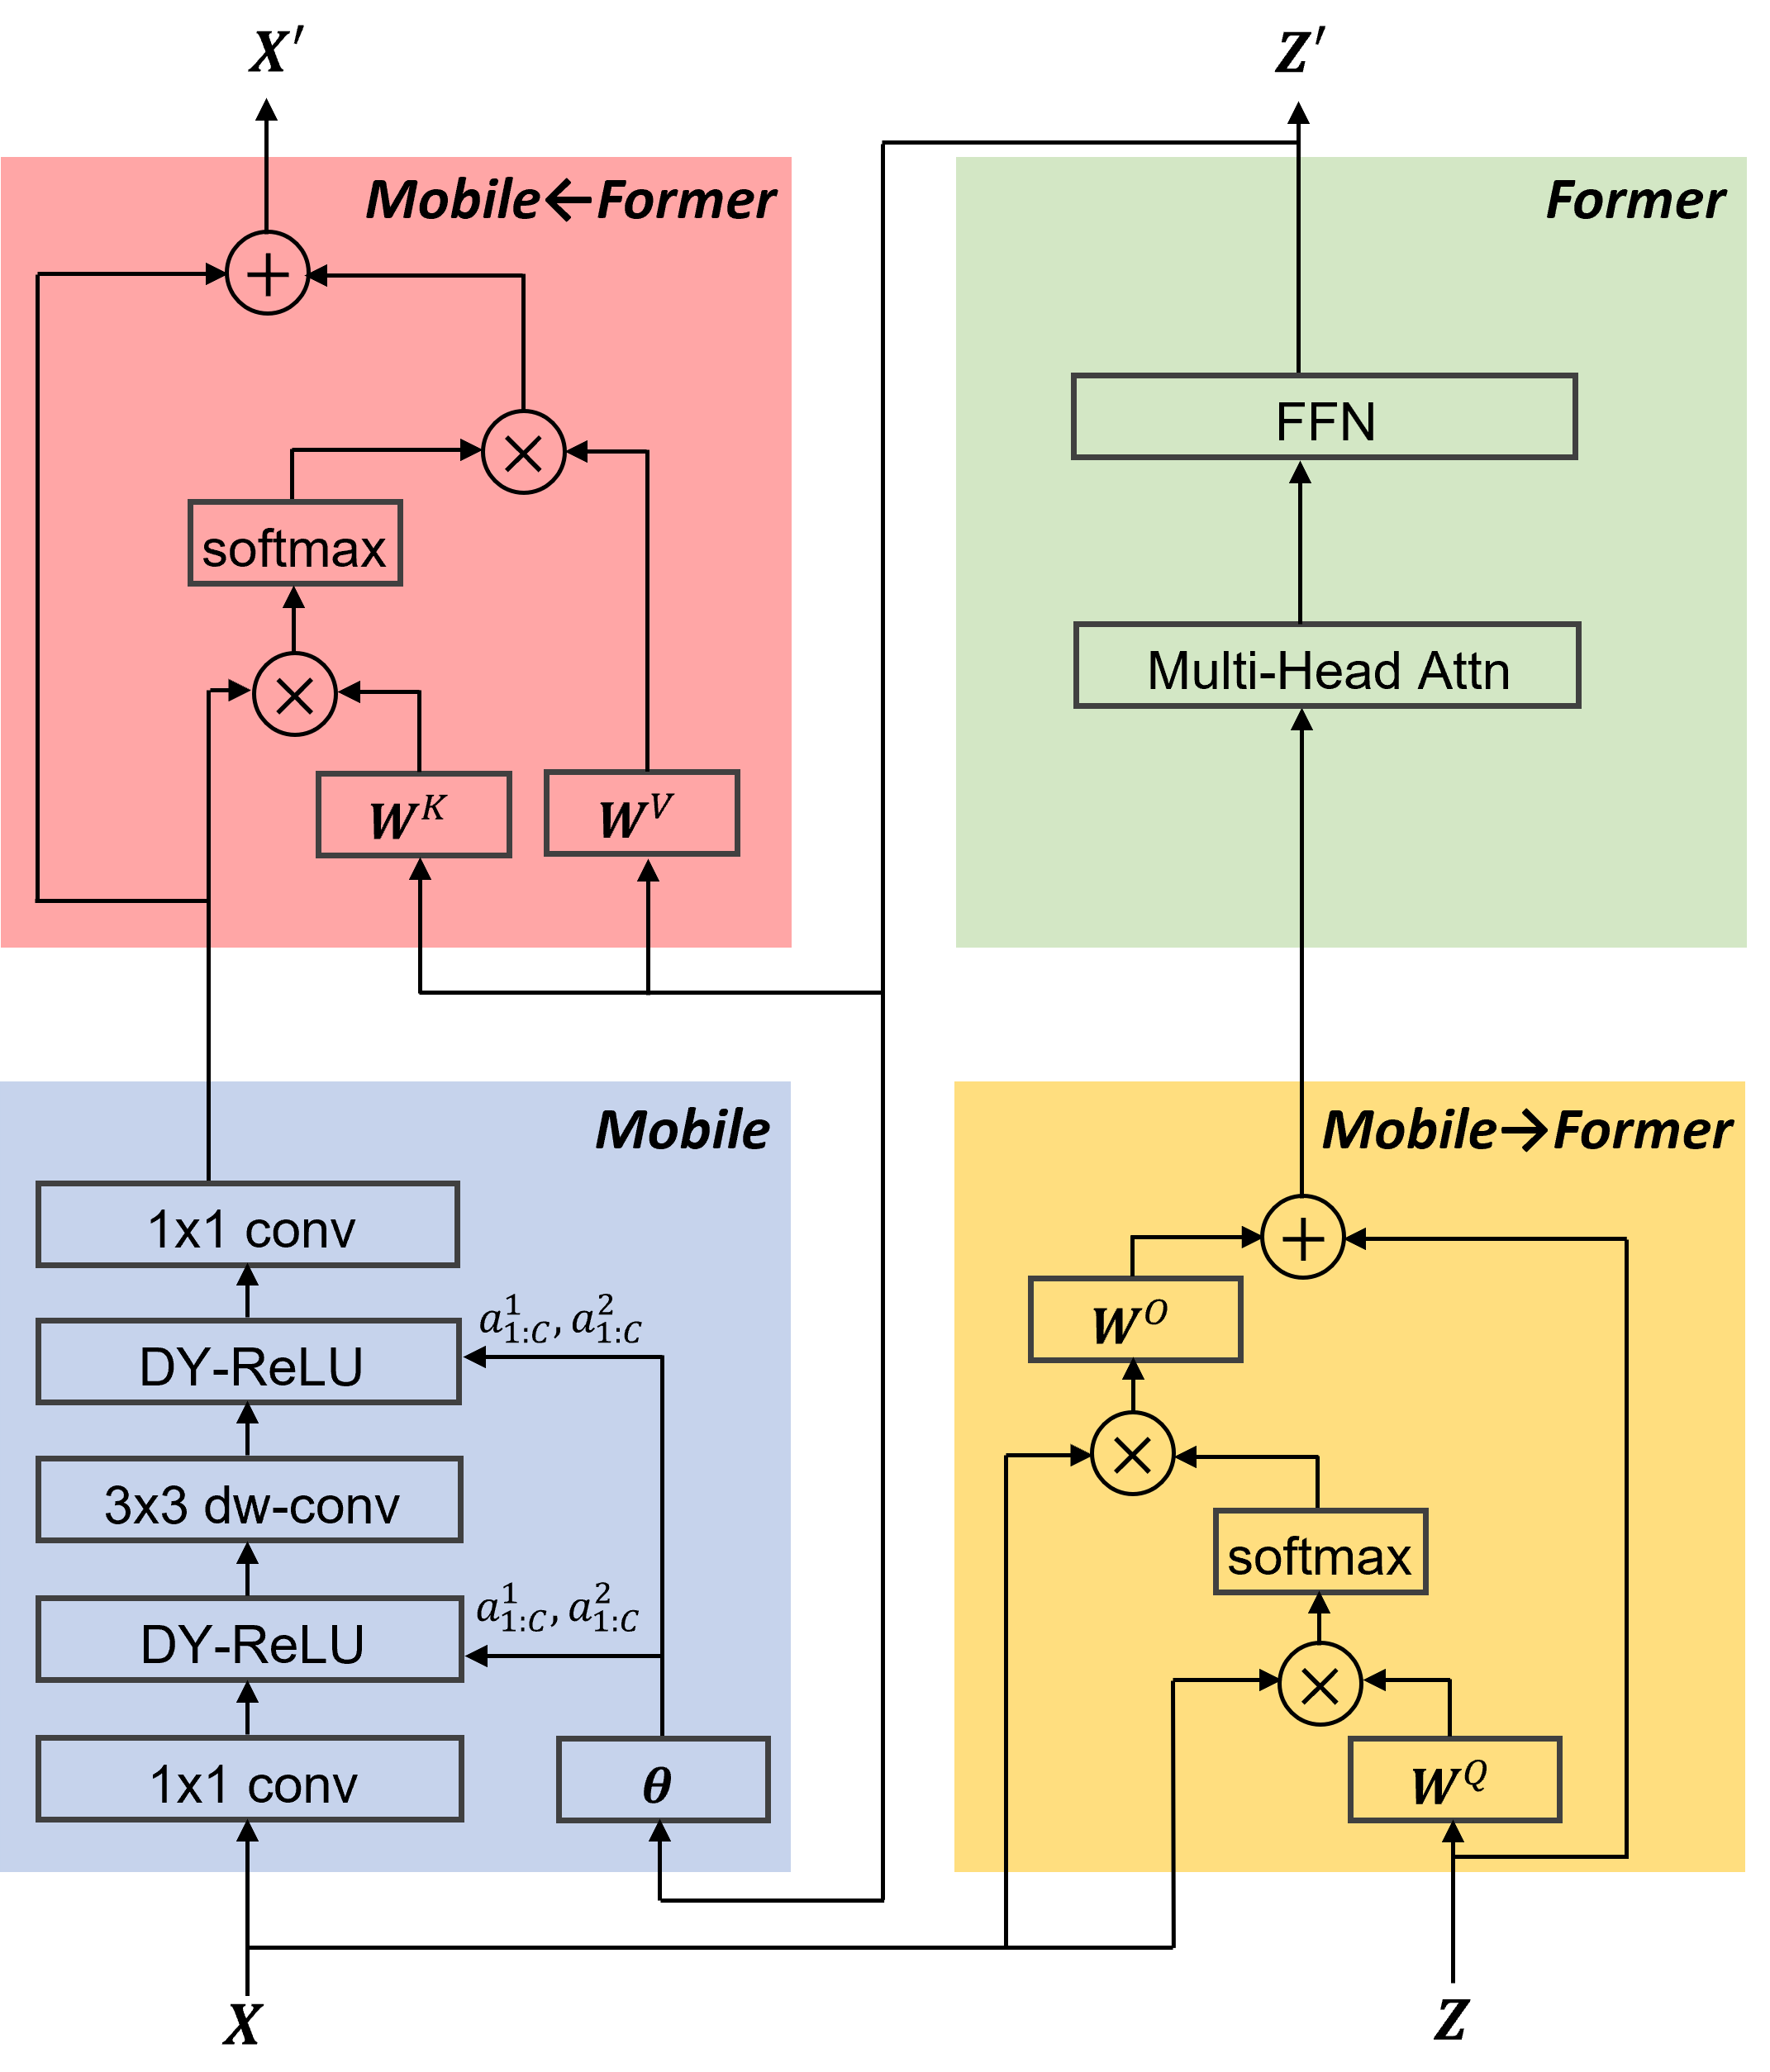
\includegraphics[width=0.36\textwidth]{images/SOTA/MobileFormerBlock.png}
    \caption{Mobile-Former Block. Fonte: \cite{chen2022mobileformerbridgingmobilenettransformer}.}
\end{figure}
Il ramo convoluzionale, che ottiene in ingresso l'intera immagine, si occupa di estrarre le \textit{features} locali, mentre il ramo basato sul meccanismo di attenzione, il quale ha in input dei token appresi, cattura le dipendenze globali. Le connessioni bidirezionali permettono a ciascun ramo di arricchire le proprie rappresentazioni con le informazioni apprese dall'altro, migliorando così la capacità complessiva del modello di comprendere sia i dettagli locali che il contesto globale dell'immagine.
Inoltre, i token utilizzati nel ramo di attenzione non sono estratti dall'immagine, come in un ViT tradizionale, ma sono appresi durante il processo di addestramento, e sono inoltre in numero molto ridotto (tipicamente 6), così da mantenere contenuto il costo computazionale dell'attenzione. Essi agiscono inizialmente da contenitori vuoti, che verranno successivamente arricchiti di informazioni provenienti dal ramo convoluzionale, e a loro volta forniranno un contesto globale che arricchirà le rappresentazioni locali di questo.
\begin{figure}[H]
    \centering
    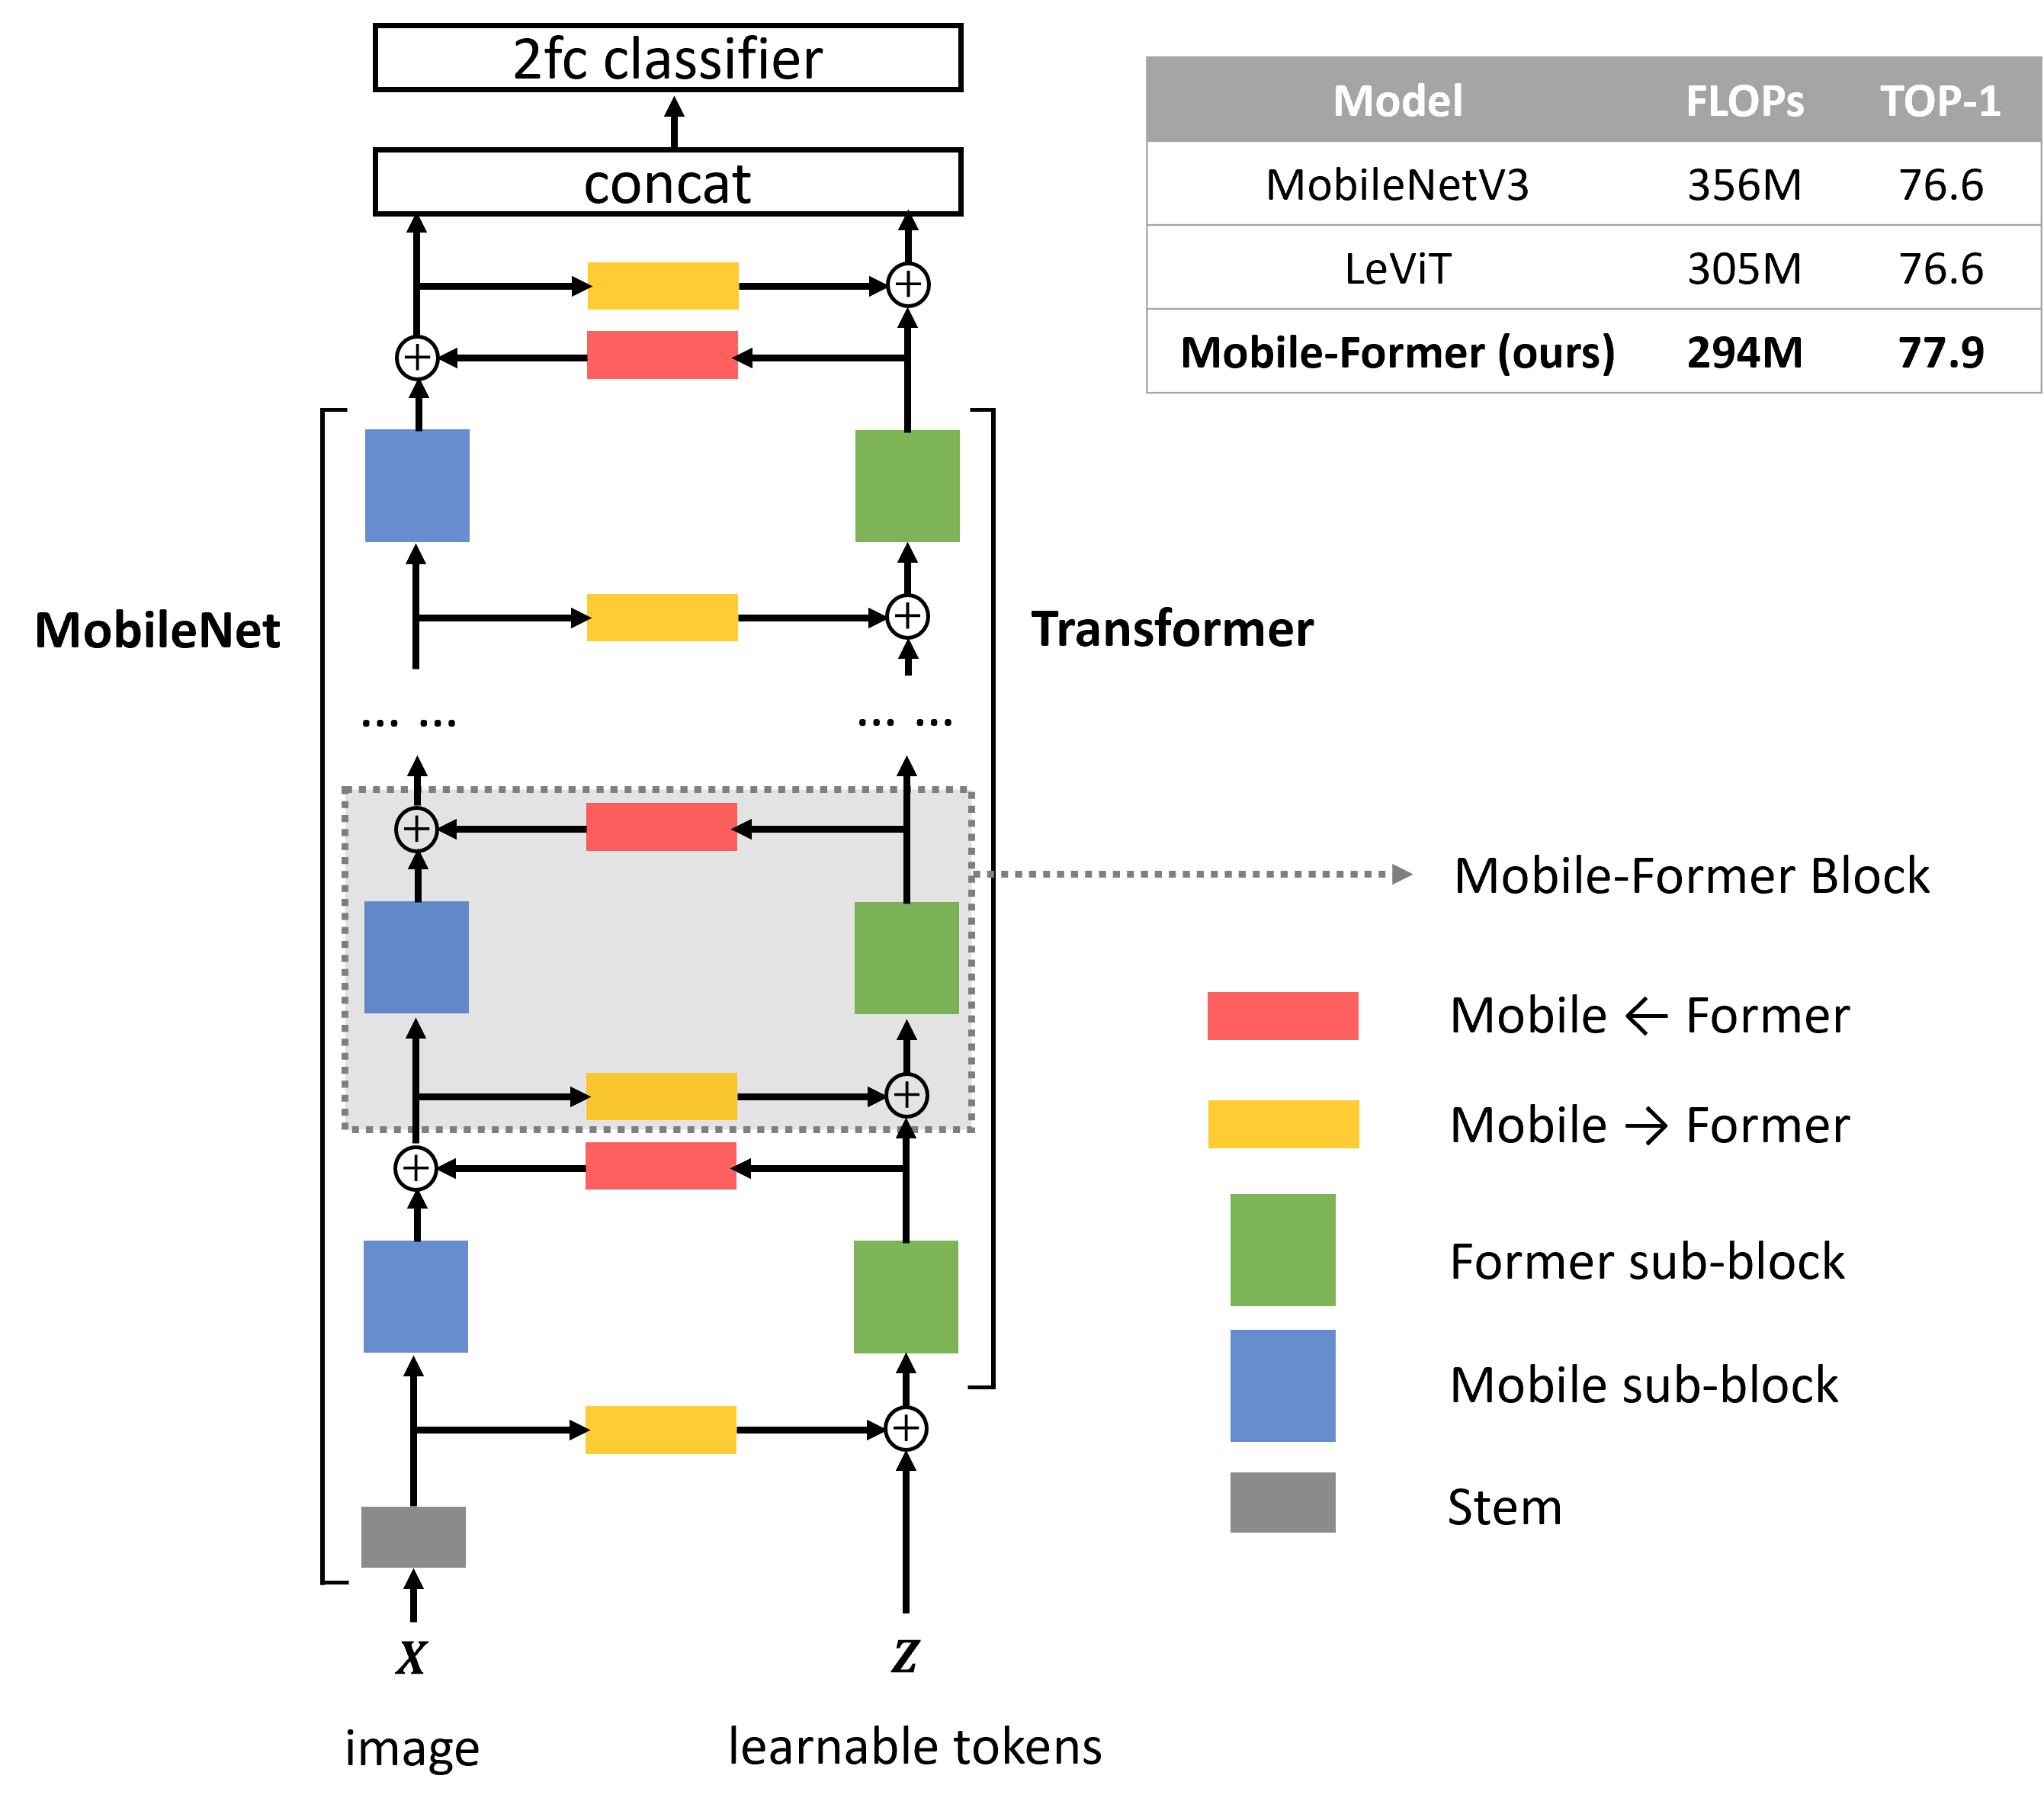
\includegraphics[width=0.6\textwidth]{images/SOTA/mobile-former.png}
    \caption{Architettura complessiva di Mobile-Former. Fonte: \cite{chen2022mobileformerbridgingmobilenettransformer}.}
\end{figure}
A valle dei blocchi \textit{Mobile-Former}, le \textit{feature map} in uscita dalla porzione convoluzionale vengono sottoposte ad una operazione di global average pooling ottenendo un vettore, a cui vengono concatenati i token del ramo di attenzione, per poi essere processati da un classificatore finale.
Grazie a questa architettura, Mobile-Former riesce a raggiungere prestazioni competitive rispetto sia ai classici modelli ViT, Swin e DeiT ma anche rispetto ad altre architetture basate su convoluzioni, con un numero di operazioni matematiche di moltiplicazione e somma (\textit{MAdds}) estremamente ridotto (circa 3-4 volte inferiori rispetto ai modelli \textit{Transformer}di riferimento), rendendolo particolarmente adatto per l'esecuzione su dispositivi mobili.
\subsubsection{EdgeViT}
Un altro esempio rilevante di architettura \textit{edge-optimized} è quello di Pan et al. \cite{pan2022edgevitscompetinglightweightcnns}, con il loro modello \textbf{EdgeViT}. Gli autori, sostenendo che \textit{MobileViT} non riesca a competere con le alternative convoluzionali ottimizzate per i dispositivi \textit{edge} in termini di compromesso tra accuratezza e complessità computazionale, propongono una nuova architettura di tipo piramidale (all'aumentare della profondità si riduce la risoluzione spaziale e aumenta il numero di canali) composta da 4 stadi che implementano un meccanismo definito \textbf{Local-Global-Local Bottleneck}, volto a ridurre il costo dell'attenzione.
\begin{figure}[H]
    \centering
    \includegraphics[width=0.75\textwidth]{images/SOTA/EdgeViT_arch.pdf}
    \caption{Architettura di EdgeViT. Fonte: \cite{pan2022edgevitscompetinglightweightcnns}.}
\end{figure}
Gli autori, partendo dal concetto di ridondanza spaziale delle immagini, che rende costosa e spesso superflua l'elaborazione di tutte le regioni dell'immagine con un meccanismo di attenzione globale, propongono una soluzione a tre fasi:
\begin{itemize}
    \item \textit{Aggregazione Locale}: per ogni token, vengono utilizzate delle convoluzioni per aggregare le informazioni provenienti da una finestra locale di dimensione fissata.
    \item \textit{Attenzione Globale Sparsa}: invece di applicare l'attenzione globale su tutti i token, vengono campionati una serie di token rappresentativi, uno per ogni finestra locale e solo su di essi viene eseguito il meccanismo di attenzione globale, riducendo drasticamente il costo computazionale.
    \item \textit{Propagazione Locale}: Vengono utilizzate delle convoluzioni trasposte per propagare le informazioni globali contenute nei token rappresentativi a tutti i token locali (all'interno della finestra). 
\end{itemize}
\begin{figure}[H]
    \centering
    \includegraphics[width=0.75\textwidth]{images/SOTA/EdgeViT_attn.pdf}
    \caption{Meccanismo di \textit{Local-Global-Local Bottleneck} applicato ad un esempio. Fonte: \cite{pan2022edgevitscompetinglightweightcnns}.}
\end{figure}
Tramite questo approccio, \textit{EdgeViT} riesce a ridurre il numero di token su cui viene calcolata l'attenzione, ma mantiene comunque la capacità di catturare dipendenze globali all'interno dell'immagine. Grazie a queste soluzioni, il modello riesce a superare le prestazioni di \textit{MobileViT} e degli altri modelli \textit{edge-optimized} e non, ottenendo un miglioramento significativo in termini di latenza. 


\subsection{Neural Architecture Search}
\section{Tecniche di compressione dei modelli}
\subsection{Quantizzazione}
\subsection{Knowledge Distillation}
\subsection{Pruning}
